\documentclass[a4paper,12pt,titlepage]{article}
\usepackage[margin=2.5cm]{geometry}
\usepackage{float,subcaption,graphicx}
\usepackage{siunitx}
\title{Digital Image Analysis - Mandatory 1}
\author{Cameron Lowell Palmer\\
	NTNU\\
	cameron.palmer@ntnu.no
}
\date{Fall 2016}

\begin{document}
\maketitle

%%%%%%%%
\section{Analyzing the textures}
Describe the 8 different textures by words. What characterizes each texture? How do the textures differ? Keywords: texture direction, frequency, variance, homogeneity, texture element size.

\begin{figure}[H]
\begin{subfigure}{0.5\textwidth}
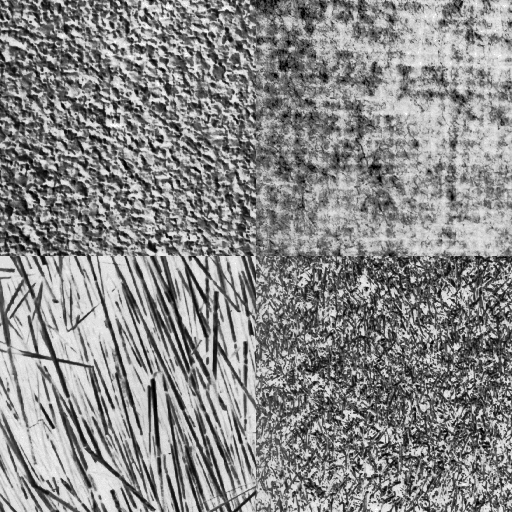
\includegraphics[width=0.9\textwidth]{textures/mosaic1}
\caption{Mosaic 1}
\label{fig:Mosaic1}
\end{subfigure}
\begin{subfigure}{0.5\textwidth}
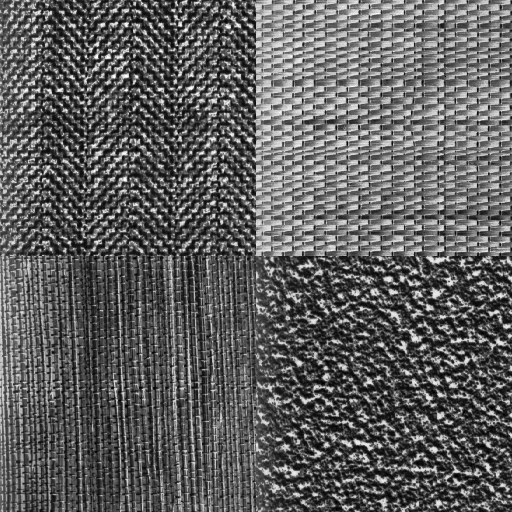
\includegraphics[width=0.9\textwidth]{textures/mosaic2}
\caption{Mosaic 2}
\label{fig:Mosaic2}
\end{subfigure}

\caption{The textures}
\label{fig:Textures}
\end{figure}

%% Mosaic 1, Top-Left Subimage and GLCM
\subsection*{Mosaic 1, Top-left}
The texture of figure \ref{fig:Mosaic1TextureTopLeft} seems to be directionally invariant and can be described as rough looking, resembling texturized concrete. The texture element size is small and relatively difficult to identify.

\begin{figure}[H]
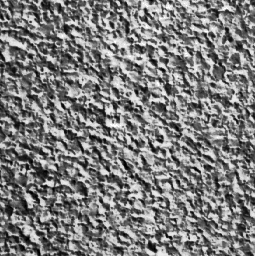
\includegraphics[width=0.4\textwidth]{textures/mosaic1-subimage-top-left}
\caption{Mosaic 1, Top-left}
\label{fig:Mosaic1TextureTopLeft}
\end{figure}

\subsection*{Mosaic 1, Top-right}
The texture in figure \ref{fig:Mosaic1TextureTopRight} looks like blotchy paper. With regular, rectangular cells running across the image with white separating lines. Possibly 20x20 cells in total. The cells are filled with medium to dark pixels.

\begin{figure}[H]
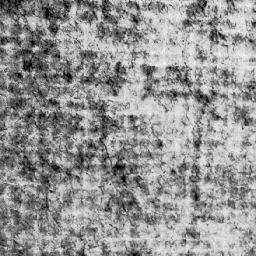
\includegraphics[width=0.4\textwidth]{textures/mosaic1-subimage-top-right}
\caption{Mosaic 1, Top-right}
\label{fig:Mosaic1TextureTopRight}
\end{figure}

\subsection*{Mosaic 1, Bottom-left}
The texture in figure \ref{fig:Mosaic1TextureBottomLeft} looks like grass running diagonally across a light gray background. The angle of the texture is quite steep, being closer to \SI{90}{\degree} than \SI{45}{\degree}. The frequency of the main texel increases as you move from the left to right-side.

\begin{figure}[H]
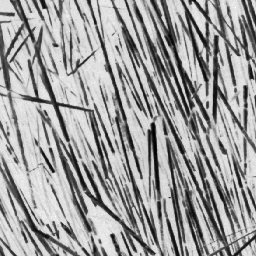
\includegraphics[width=0.4\textwidth]{textures/mosaic1-subimage-bottom-left}
\caption{Mosaic 1, Bottom-left}
\label{fig:Mosaic1TextureBottomLeft}
\end{figure}

\subsection*{Mosaic 1, Bottom-right}
The texture in figure \ref{fig:Mosaic1TextureBottomRight} is similar to figure \ref{fig:Mosaic1TextureTopLeft} although the texels are smaller and rather than resembling rough concrete are more like looking at very dense black-and-white tree foliage from a high altitude. Again, I would describe this texture as direction invariant.

\begin{figure}[H]
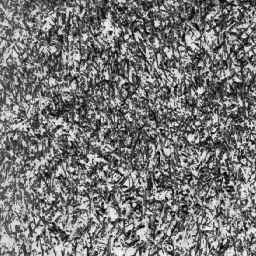
\includegraphics[width=0.4\textwidth]{textures/mosaic1-subimage-bottom-right}
\caption{Mosaic 1, Bottom-right}
\label{fig:Mosaic1TextureBottomRight}
\end{figure}


%% Mosaic 2, Top-Left Subimage and GLCM
\subsection*{Mosaic 2, Top-left}
The texture in figure \ref{fig:Mosaic2TextureTopLeft} is definitely a fabric with a weave running at alternating \SI{45}{\degree} angles. Around three cycles of direction change are visible. Mostly dark, but with specks of white spread fairly evenly across the subimage.

\begin{figure}[H]
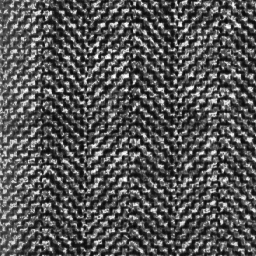
\includegraphics[width=0.4\textwidth]{textures/mosaic2-subimage-top-left}
\caption{Mosaic 2, Top-left}
\label{fig:Mosaic2TextureTopLeft}
\end{figure}

\subsection*{Mosaic 2, Top-right}
The texture in figure \ref{fig:Mosaic2TextureTopRight} is quite likely a woven natural grass fiber mat. The overall direction is a left-right, top-bottom grid patter of fairly consistently sized rectangles, possibly 60x40 in size. The color seems to alternate across the cells from light to dark gray.

\begin{figure}[H]
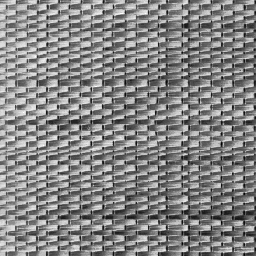
\includegraphics[width=0.4\textwidth]{textures/mosaic2-subimage-top-right}
\caption{Mosaic 2, Top-right}
\label{fig:Mosaic2TextureTopRight}
\end{figure}

\subsection*{Mosaic 2, Bottom-left}
The texture in figure \ref{fig:Mosaic2TextureBottomLeft} is less directly identifiable, but like figure \ref{fig:Mosaic1TextureTopRight} seems to be some sort of natural fiber. It is clearly comprised of smaller texels than \ref{fig:Mosaic1TextureTopRight} and a tight wavy pattern that runs left-to-right. Each wave is cut or notched from top to bottom at a regular interval. Overall color is pretty dark.

\begin{figure}[H]
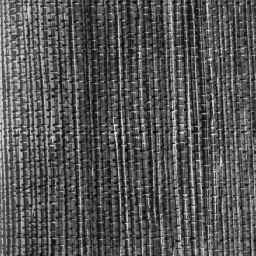
\includegraphics[width=0.4\textwidth]{textures/mosaic2-subimage-bottom-left}
\caption{Mosaic 2, Bottom-left}
\label{fig:Mosaic2TextureBottomLeft}
\end{figure}

\subsection*{Mosaic 2, Bottom-right}
The texture in figure \ref{fig:Mosaic2TextureBottomRight} is a darker version of figure \ref{fig:Mosaic1TextureTopLeft} and looking a little smoother.

\begin{figure}[H]
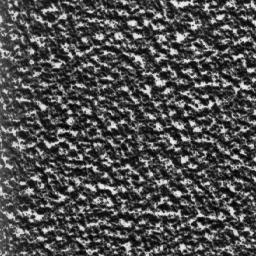
\includegraphics[width=0.4\textwidth]{textures/mosaic2-subimage-bottom-right}
\caption{Mosaic 2, Bottom-right}
\label{fig:Mosaic2TextureBottomRight}
\end{figure}

%%%%%%%%
\section{Visualizing GLCM matrices}
For the project I have chosen to use 16 gray-levels and a window size of 31 with a directional offset of 2. I chose the window size largely related to the general feature size contained within the texture. I think this is a good size that will adequately extract the textures although a smaller window size might do a better job of identifying the boundary.

The textures diagonal from each other in \ref{fig:Mosaic1}, top-left, bottom-right, and top-right, bottom-left seem the most similar and in \ref{fig:Mosaic2}, the top-left and bottom-right. This similarity will make it difficult to separate the textures in a clean way.

%% Mosaic 1, Top-left Subimage and GLCMs
\subsection{Mosaic 1, Top-left}
All three angles I tried yielded nearly identical results backing up my direction invariance claim. Mostly concentrated along the diagonal and towards 0-0 and 255-255.

\begin{figure}[H]
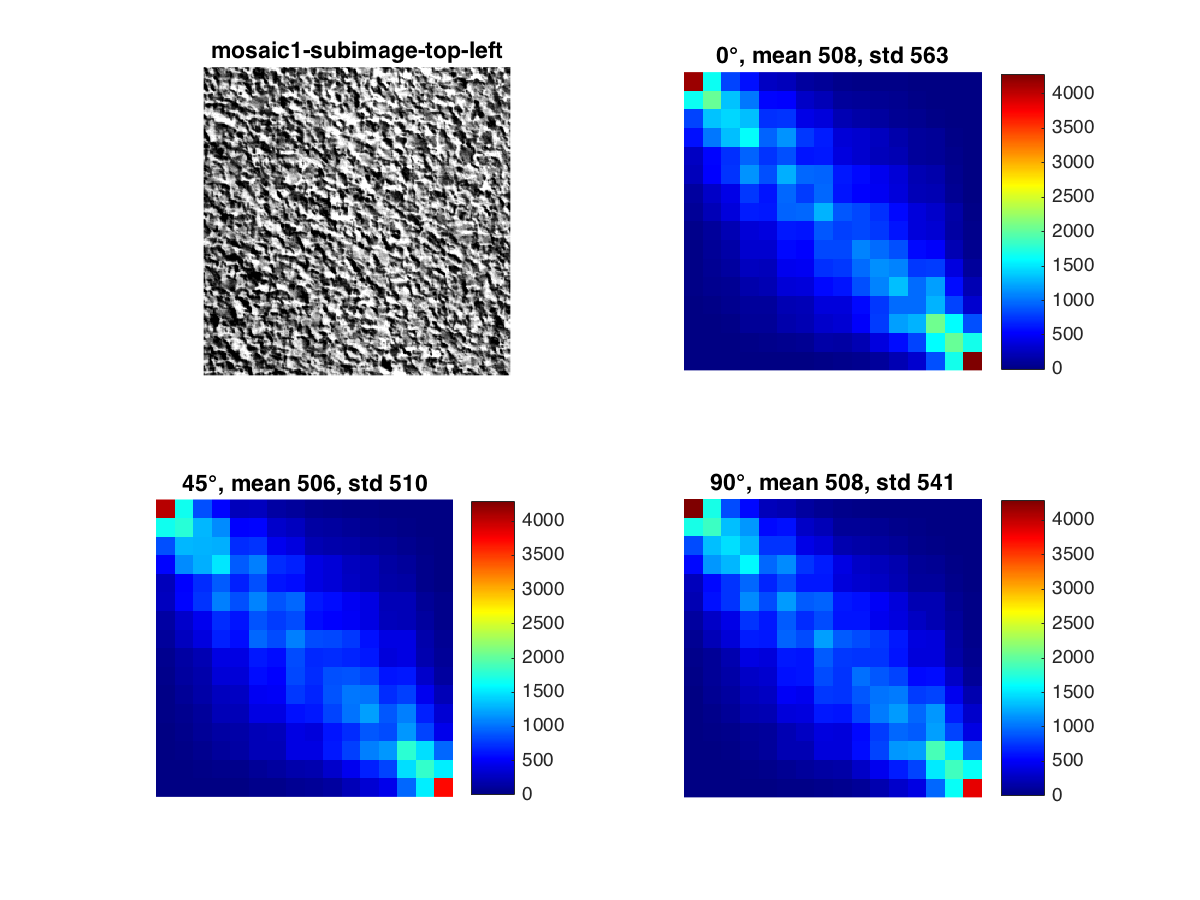
\includegraphics[width=0.7\textwidth]{partB-mosaic1-subimage-top-left}
\caption{Mosaic 1, Top-left}
\label{fig:Mosaic1SubimageTopLeft}
\end{figure}

%% Mosaic 1, Top-right Subimage and GLCMs
\subsection{Mosaic 1, Top-right}
\begin{figure}[H]
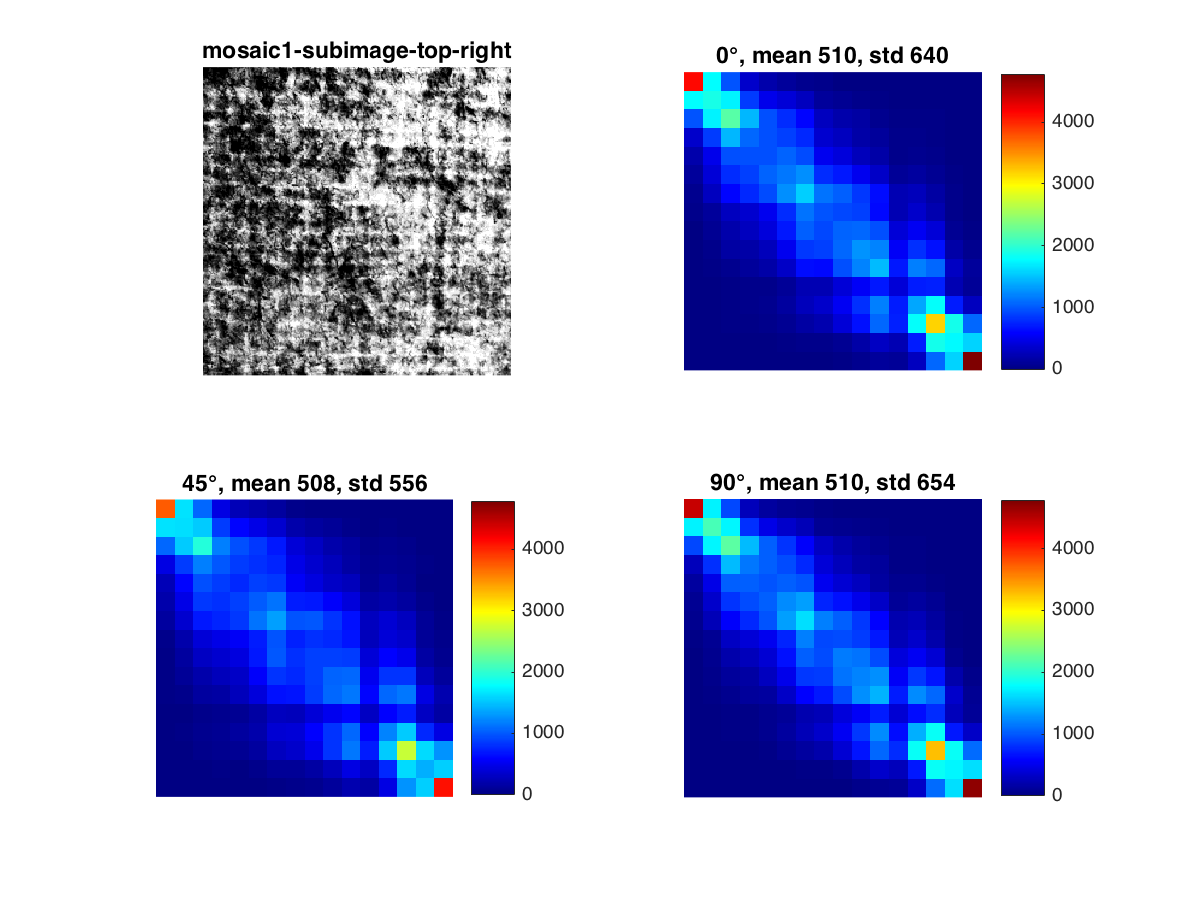
\includegraphics[width=0.9\textwidth]{partB-mosaic1-subimage-top-right}
\caption{Mosaic 1, Top-right}
\label{fig:Mosaic1SubimageTopRight}
\end{figure}

%% Mosaic 1, Bottom-left Subimage and GLCMs
\subsection{Mosaic 1, Bottom-left}
\begin{figure}[H]
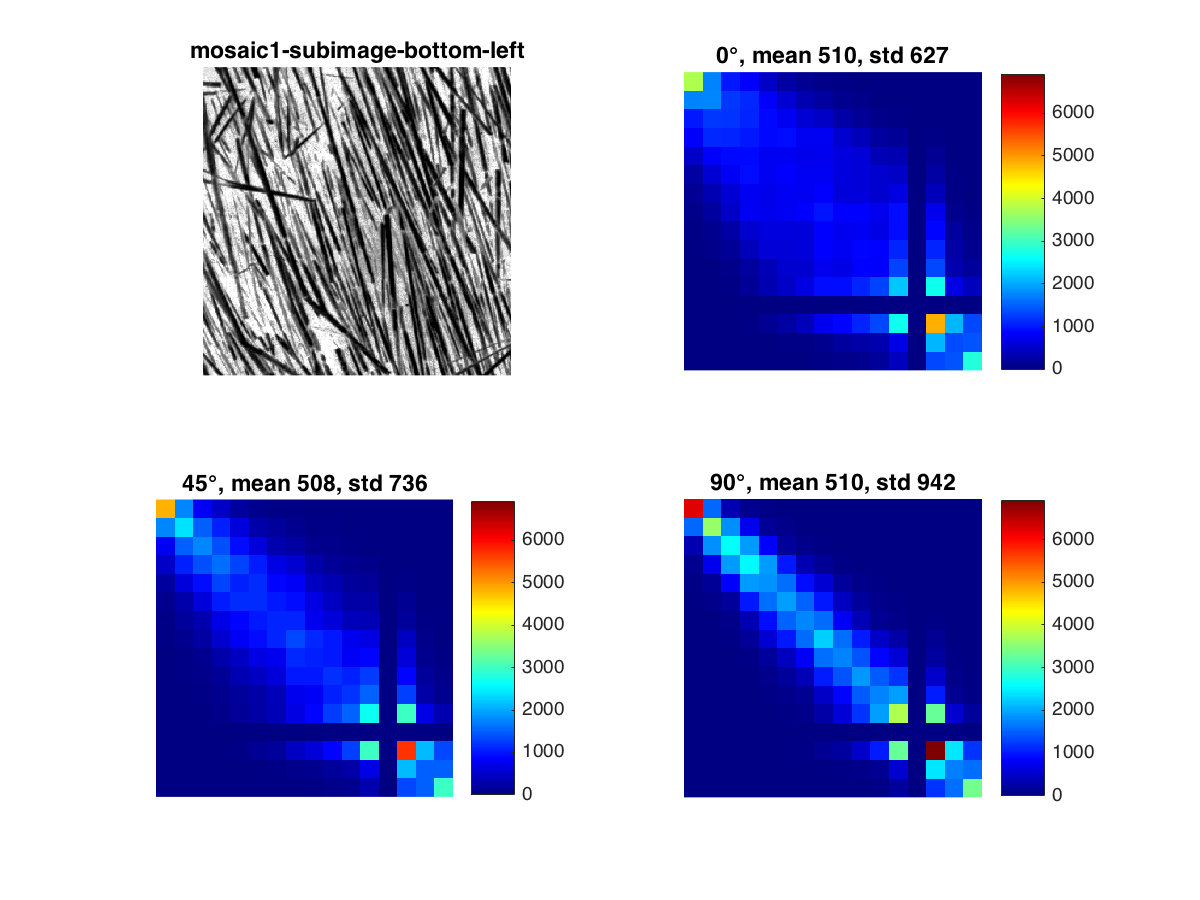
\includegraphics[width=0.9\textwidth]{partB-mosaic1-subimage-bottom-left}
\caption{Mosaic 1, Bottom-left}
\label{fig:Mosaic1SubimageBottomLeft}
\end{figure}

%% Mosaic 1, Bottom-right Subimage and GLCMs
\subsection{Mosaic 1, Bottom-right}
\begin{figure}[H]
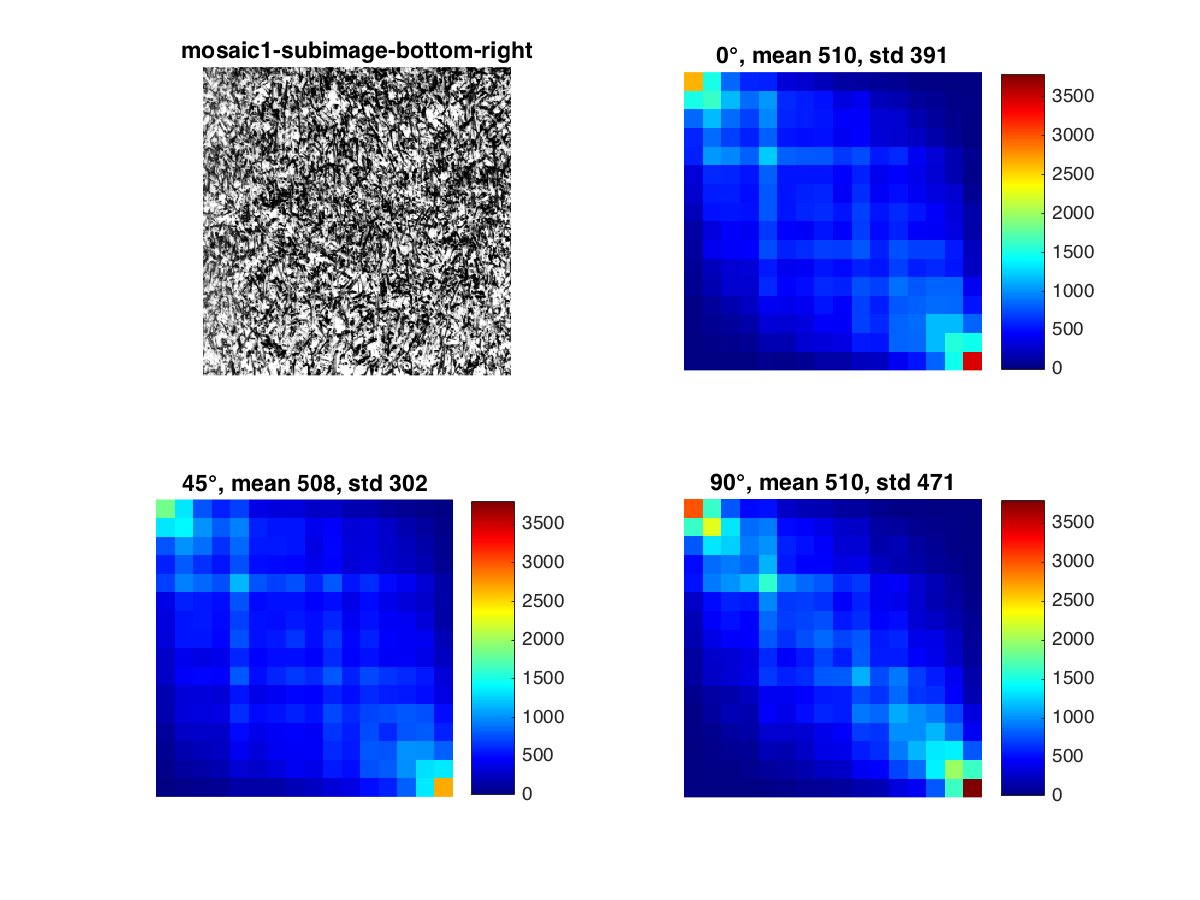
\includegraphics[width=0.9\textwidth]{partB-mosaic1-subimage-bottom-right}
\caption{Mosaic 1, Bottom-right}
\label{fig:Mosaic1SubimageBottomRight}
\end{figure}

%% Mosaic 2, Top-left Subimage and GLCMs
\subsection{Mosaic 2, Top-left}
\begin{figure}[H]
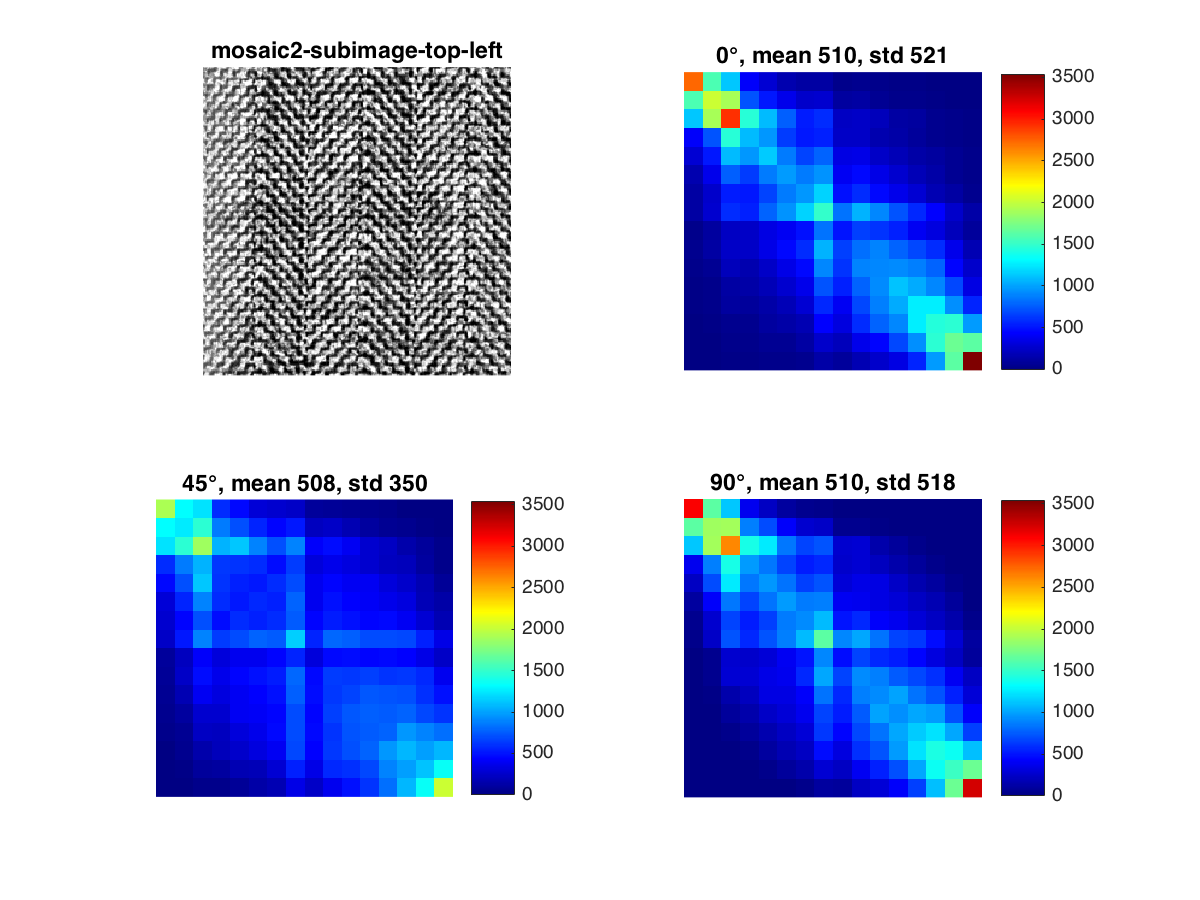
\includegraphics[width=0.9\textwidth]{partB-mosaic2-subimage-top-left}
\caption{Mosaic 2, Top-left}
\label{fig:Mosaic2SubimageTopLeft}
\end{figure}

%% Mosaic 2, Top-right Subimage and GLCMs
\subsection{Mosaic 2, Top-right}
\begin{figure}[H]
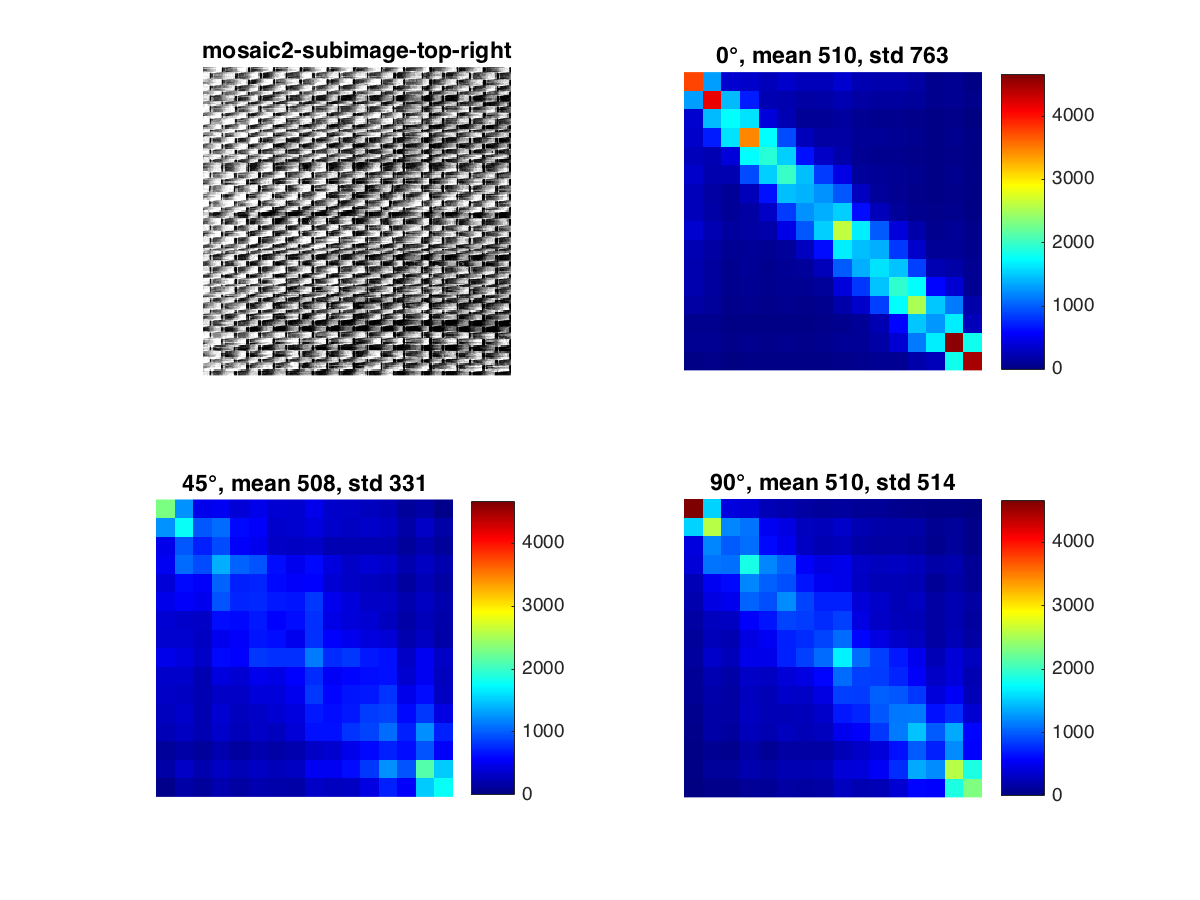
\includegraphics[width=0.9\textwidth]{partB-mosaic2-subimage-top-right}
\caption{Mosaic 2, Top-right}
\label{fig:Mosaic2SubimageTopRight}
\end{figure}

%% Mosaic 2, Bottom-left Subimage and GLCMs
\subsection{Mosaic 2, Bottom-left}
\begin{figure}[H]
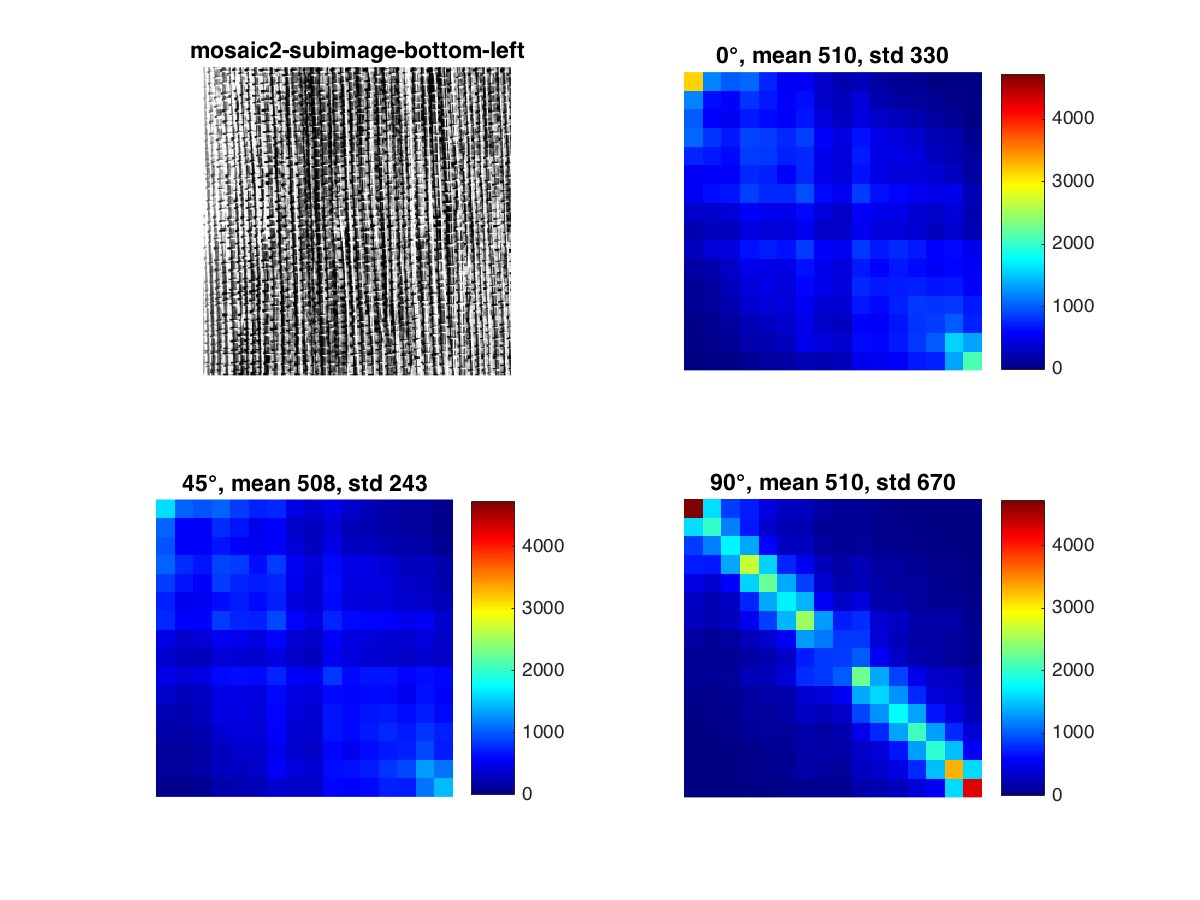
\includegraphics[width=0.9\textwidth]{partB-mosaic2-subimage-bottom-left}
\caption{Mosaic 2, Bottom-left}
\label{fig:Mosaic2SubimageBottomLeft}
\end{figure}

%% Mosaic 2, Bottom-right Subimage and GLCMs
\subsection{Mosaic 2, Bottom-right}
\begin{figure}[H]
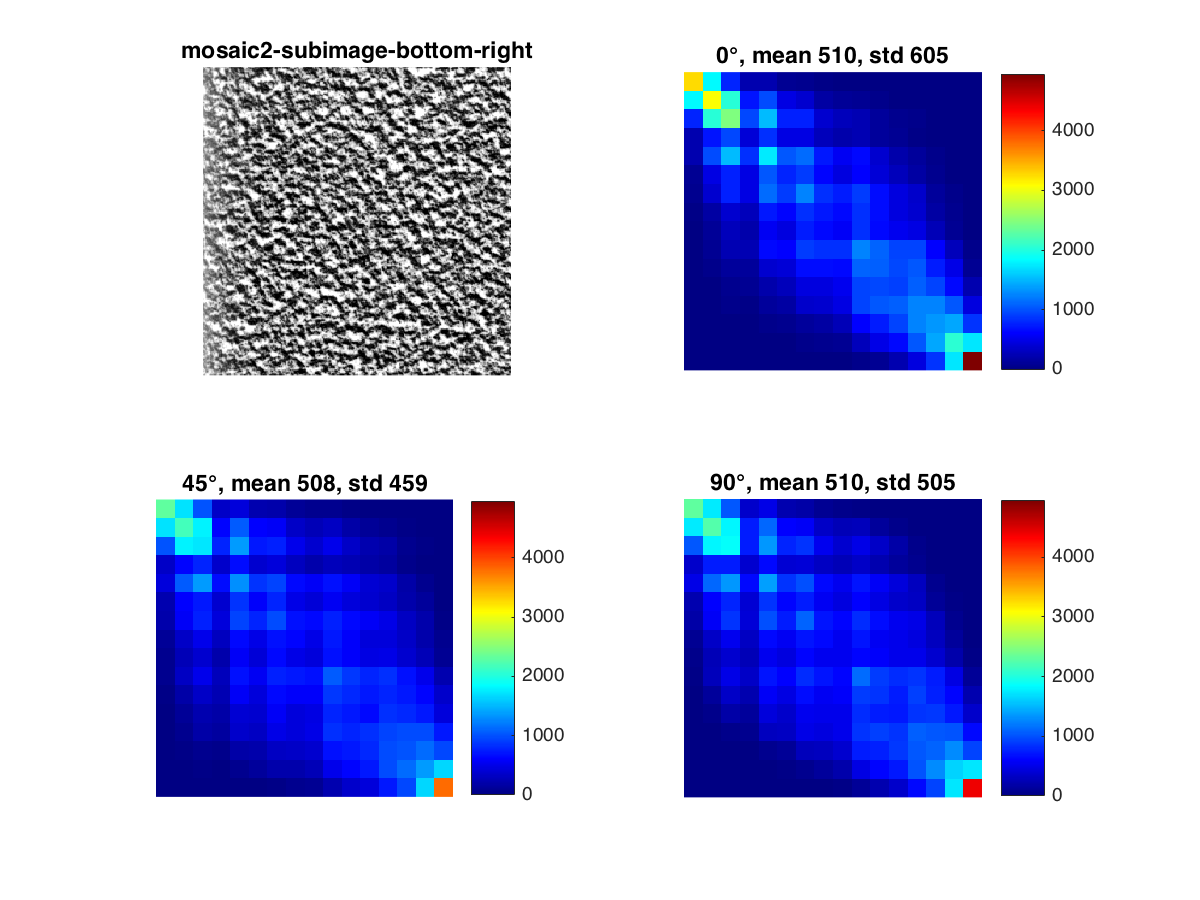
\includegraphics[width=0.9\textwidth]{partB-mosaic2-subimage-bottom-right}
\caption{Mosaic 2, Bottom-right}
\label{fig:Mosaic2SubimageBottomRight}
\end{figure}

%%%%%%%%
\section{Computing GLCM feature images in local windows}

Window size was chosen mostly based on the overall size of the image and the subimage texture size. Given that the images are 512x512 pixels and the subimages take up a quarter of each image a window size of 31 seemed reasonable. I computed each of the GLCM features at \SI{0}{\degree}, \SI{45}{\degree}, and \SI{90}{\degree} angles.

%% Mosaic 1
\subsection{Mosaic 1, Angle 0}
\begin{figure}[H]
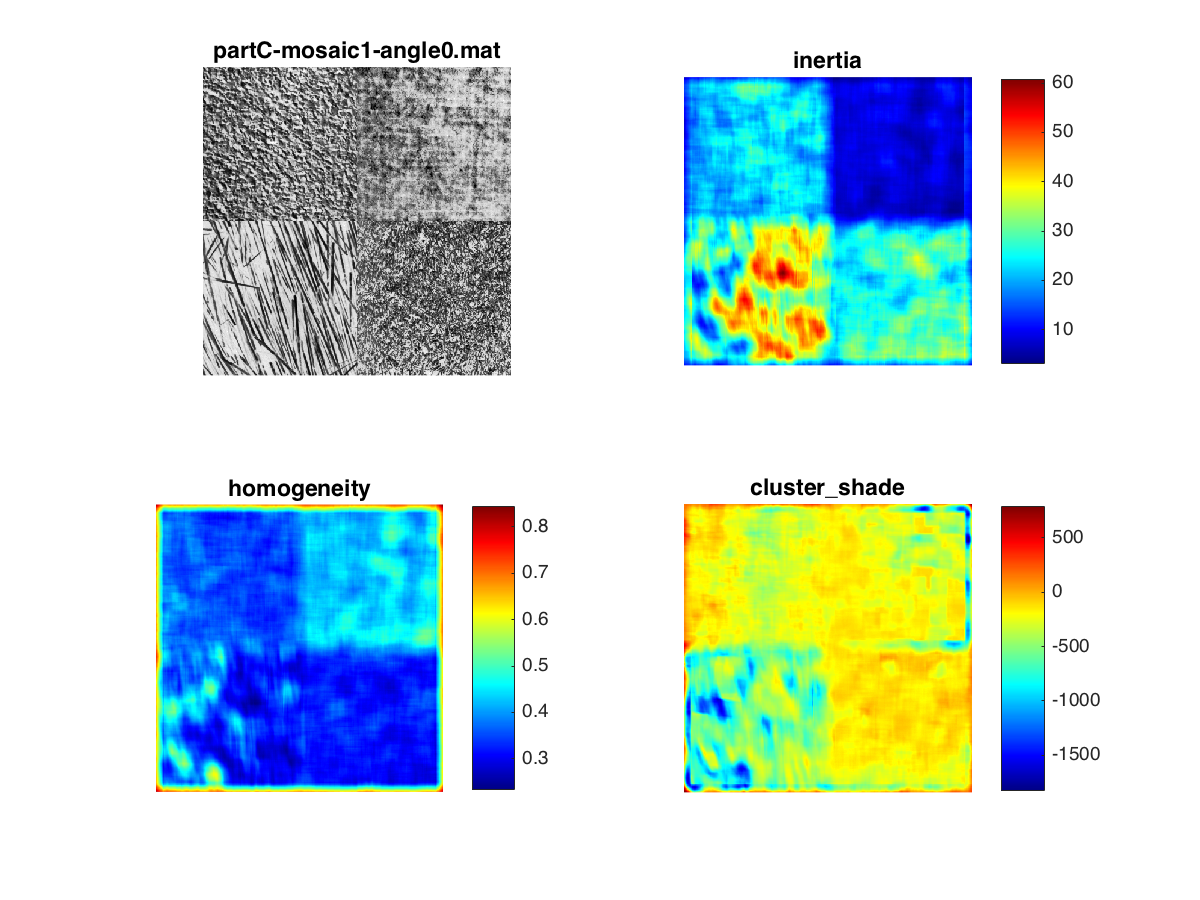
\includegraphics[width=0.8\textwidth]{partC-mosaic1-angle0}
\caption{Mosaic 1, Angle 0}
\label{fig:Mosaic1Angle0}
\end{figure}

\subsection{Mosaic 1, Angle 45}
\begin{figure}[H]
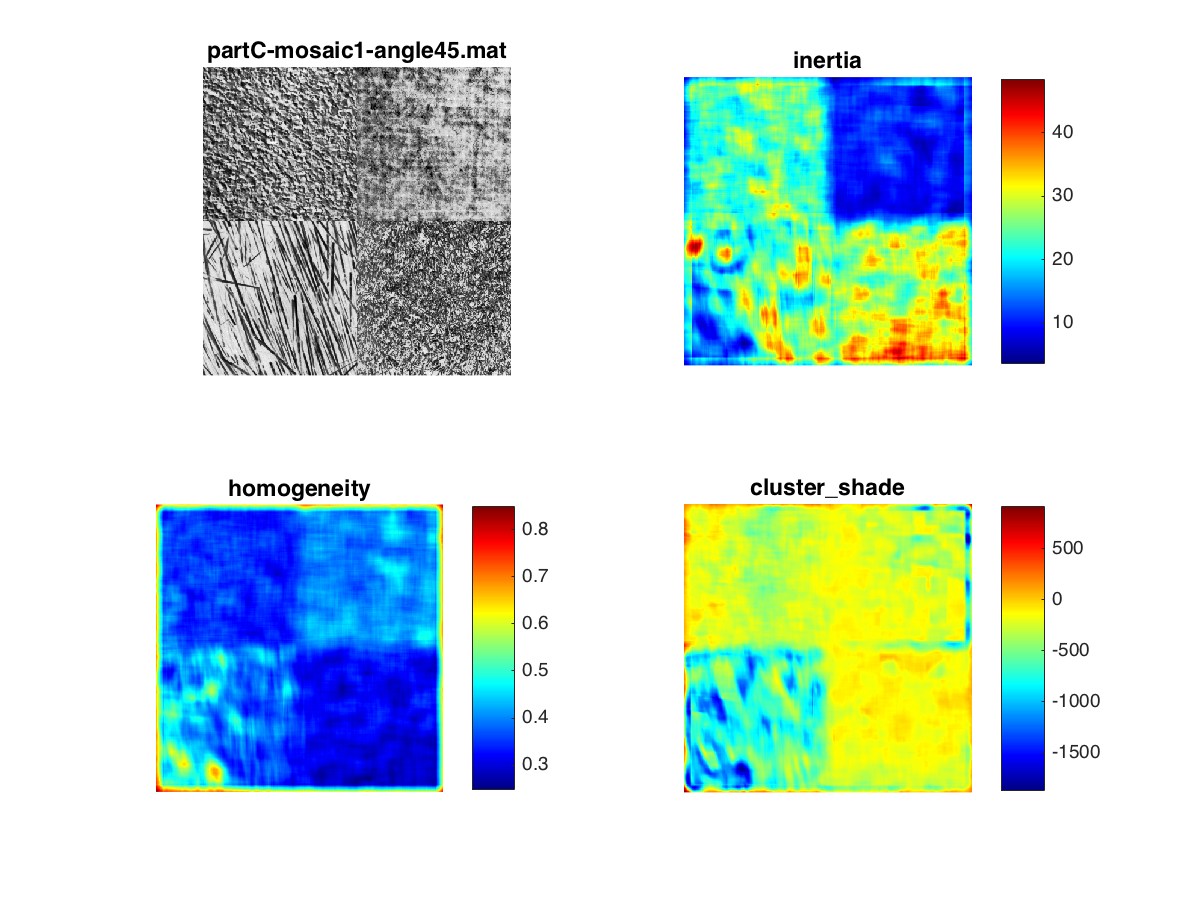
\includegraphics[width=0.8\textwidth]{partC-mosaic1-angle45}
\caption{Mosaic 1, Angle 45}
\label{fig:Mosaic1Angle45}
\end{figure}

\subsection{Mosaic 1, Angle 90}
\begin{figure}[H]
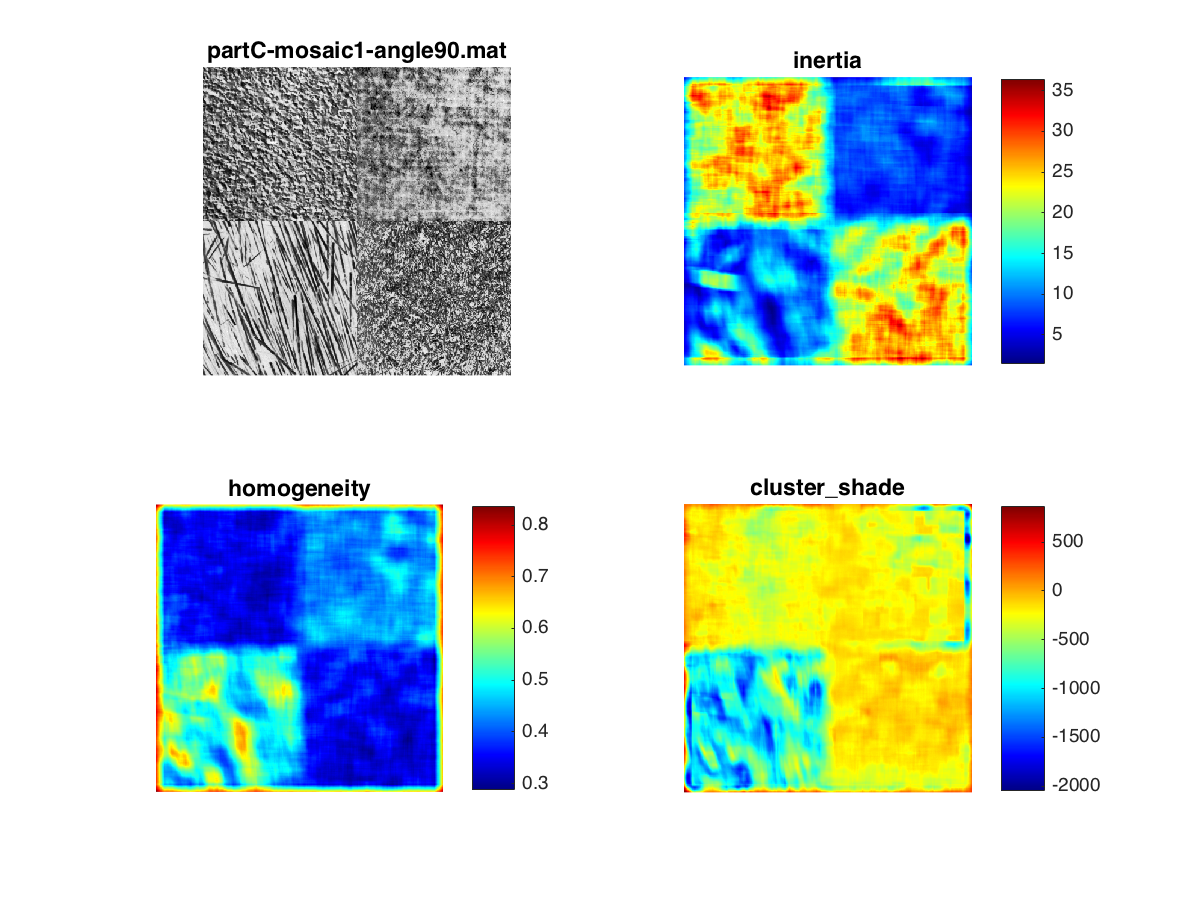
\includegraphics[width=0.8\textwidth]{partC-mosaic1-angle90}
\caption{Mosaic 1, Angle 90}
\label{fig:Mosaic1Angle90}
\end{figure}

%% Mosaic 2
\subsection{Mosaic 2, Angle 0}
\begin{figure}[H]
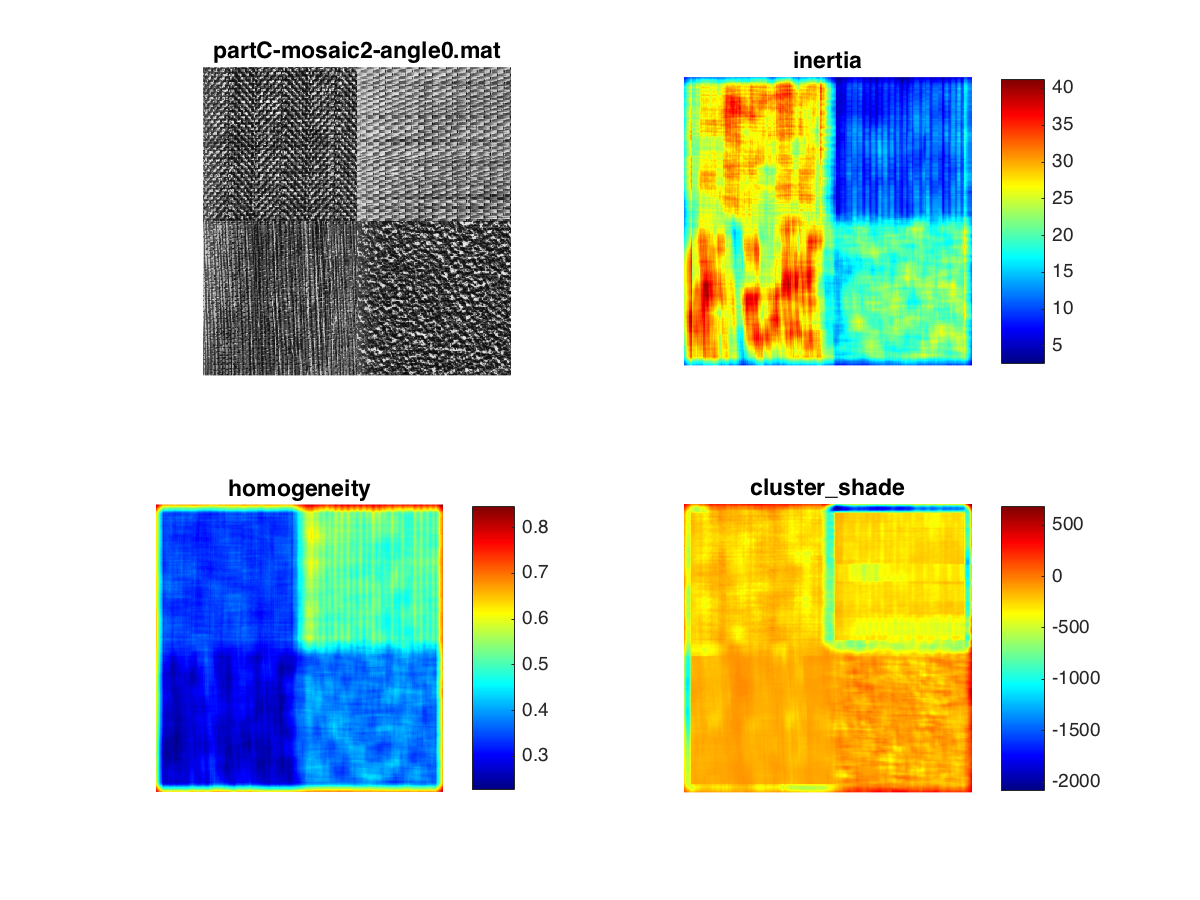
\includegraphics[width=0.8\textwidth]{partC-mosaic2-angle0}
\caption{Mosaic 2, Angle 0}
\label{fig:Mosaic2Angle0}
\end{figure}

\subsection{Mosaic 2, Angle 45}
\begin{figure}[H]
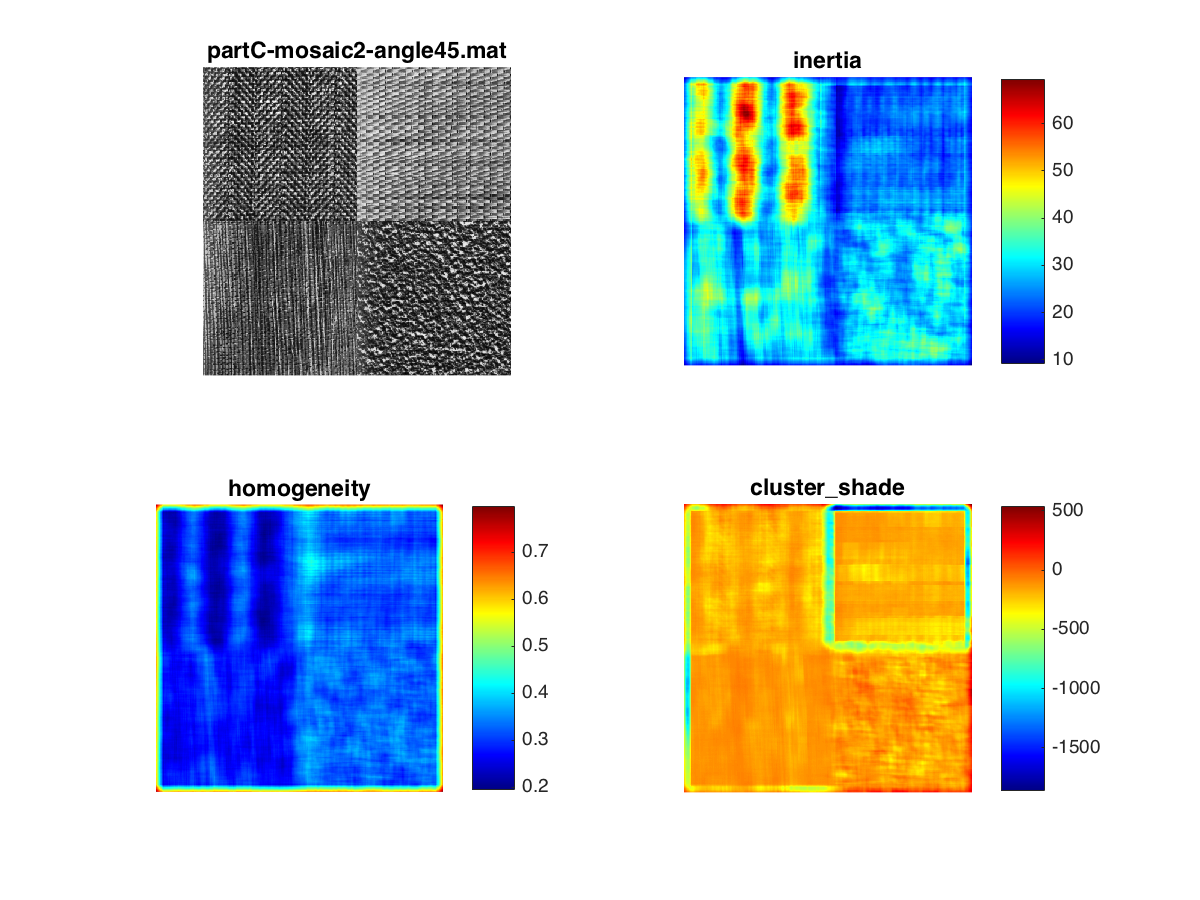
\includegraphics[width=0.8\textwidth]{partC-mosaic2-angle45}
\caption{Mosaic 2, Angle 45}
\label{fig:Mosaic2Angle45}
\end{figure}

\subsection{Mosaic 2, Angle 90}
\begin{figure}[H]
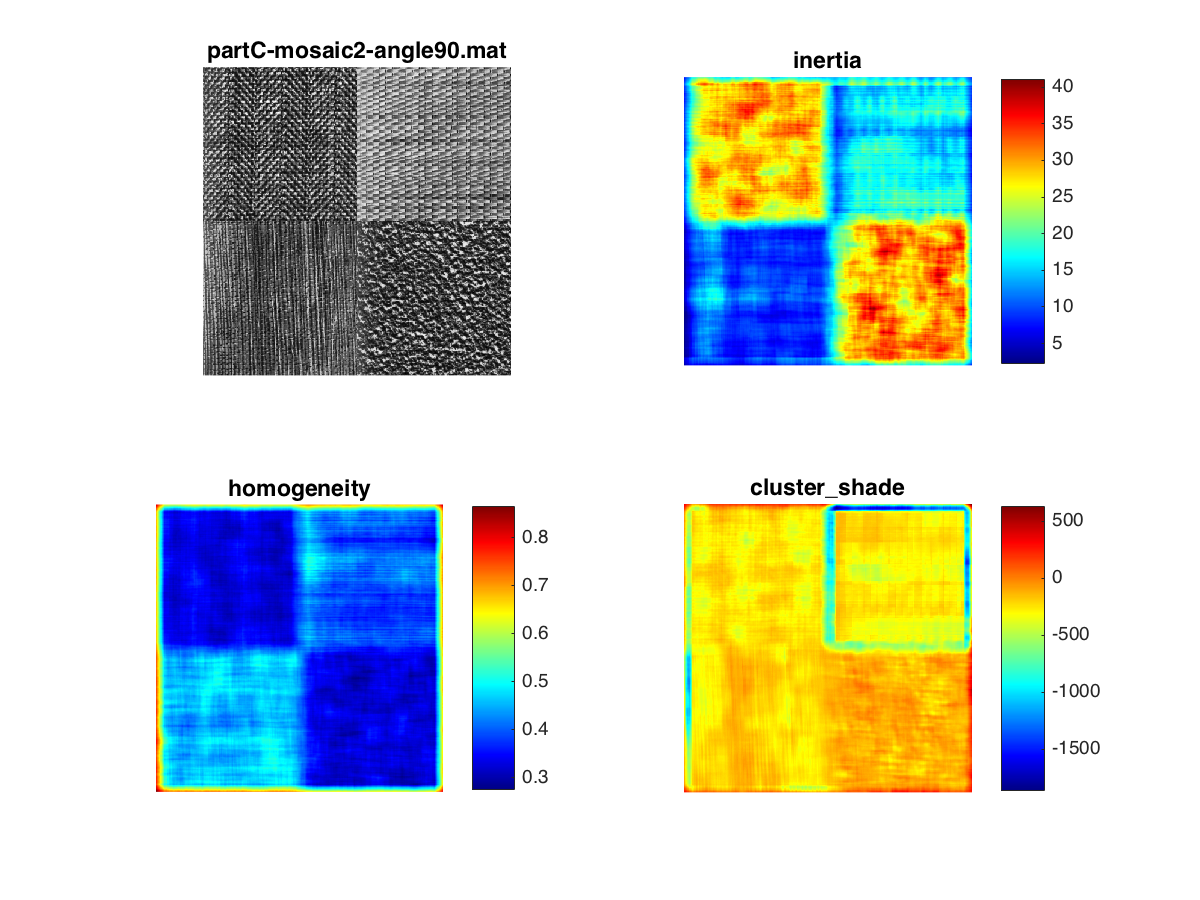
\includegraphics[width=0.8\textwidth]{partC-mosaic2-angle90}
\caption{Mosaic 2, Angle 90}
\label{fig:Mosaic2Angle90}
\end{figure}

%%%%%%%%
\section{Segment the GLCM feature images and describe how they separate the textures}

Generally I used only a couple of angles and a specific combination of GLCM features to extract the subimages. In both mosaics I first used homogeneity to isoloate the two diagonal subimages and then simply flipped the thresholding to isolate the other pair. Then it became a matter of separating each pair using a different feature to break apart the pair.

\subsection*{Mosaic 1, Top-left}
Segment \ref{fig:Mosaic1SegmentedTopLeft}. Segmented using homogeneity at .40 and a \SI{90}{\degree} angle, followed by intertia at 13 using a \SI{45}{\degree} angle.

\begin{figure}[H]
	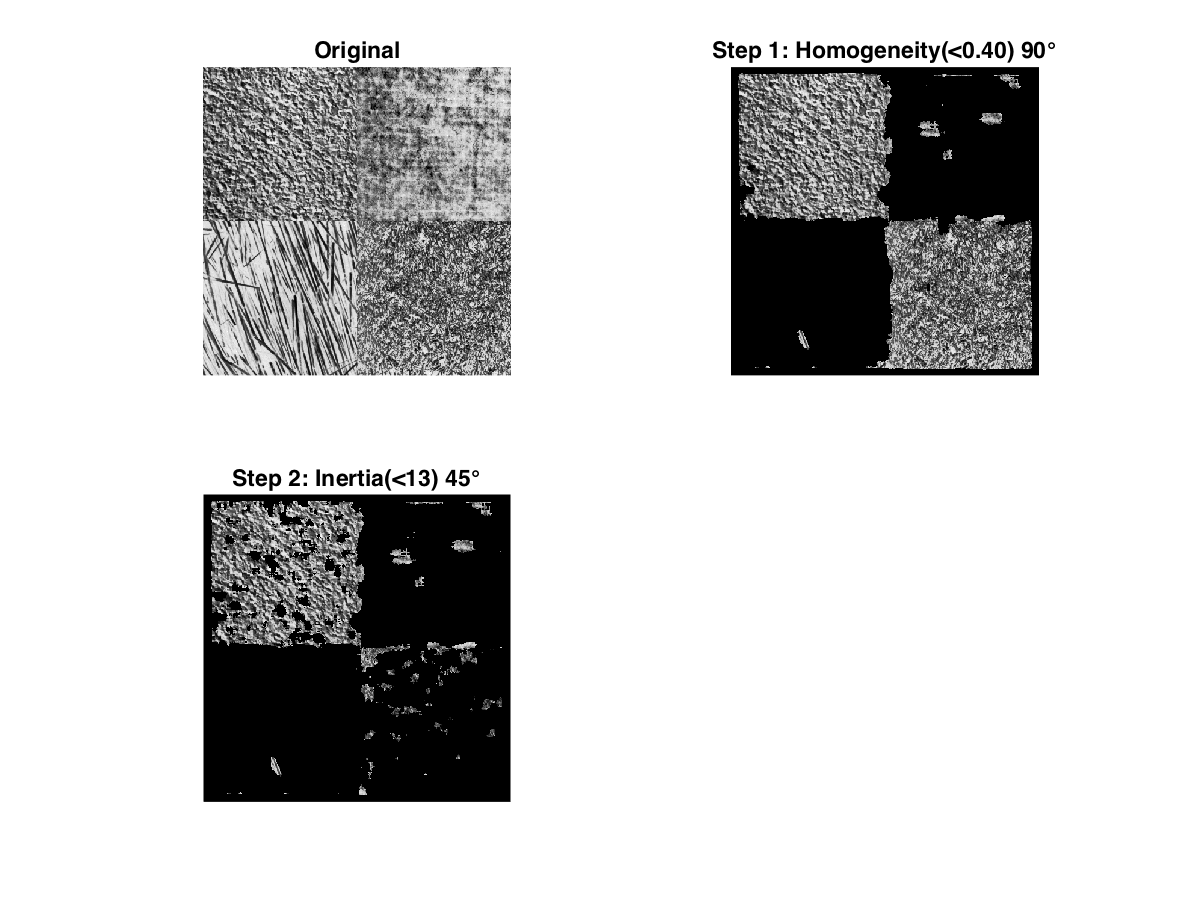
\includegraphics[width=0.8\textwidth]{partD-mosaic1-segmentation-top-left}
	\caption{Mosaic 1, top-left}
	\label{fig:Mosaic1SegmentedTopLeft}
\end{figure}

\subsection*{Mosaic 1, Top-right} 
Segment \ref{fig:Mosaic1SegmentedTopRight}. Segmented using homogeneity at .40 and a \SI{90}{\degree} angle, followed by cluster shade at -400 using a \SI{45}{\degree} angle.

\begin{figure}[H]
	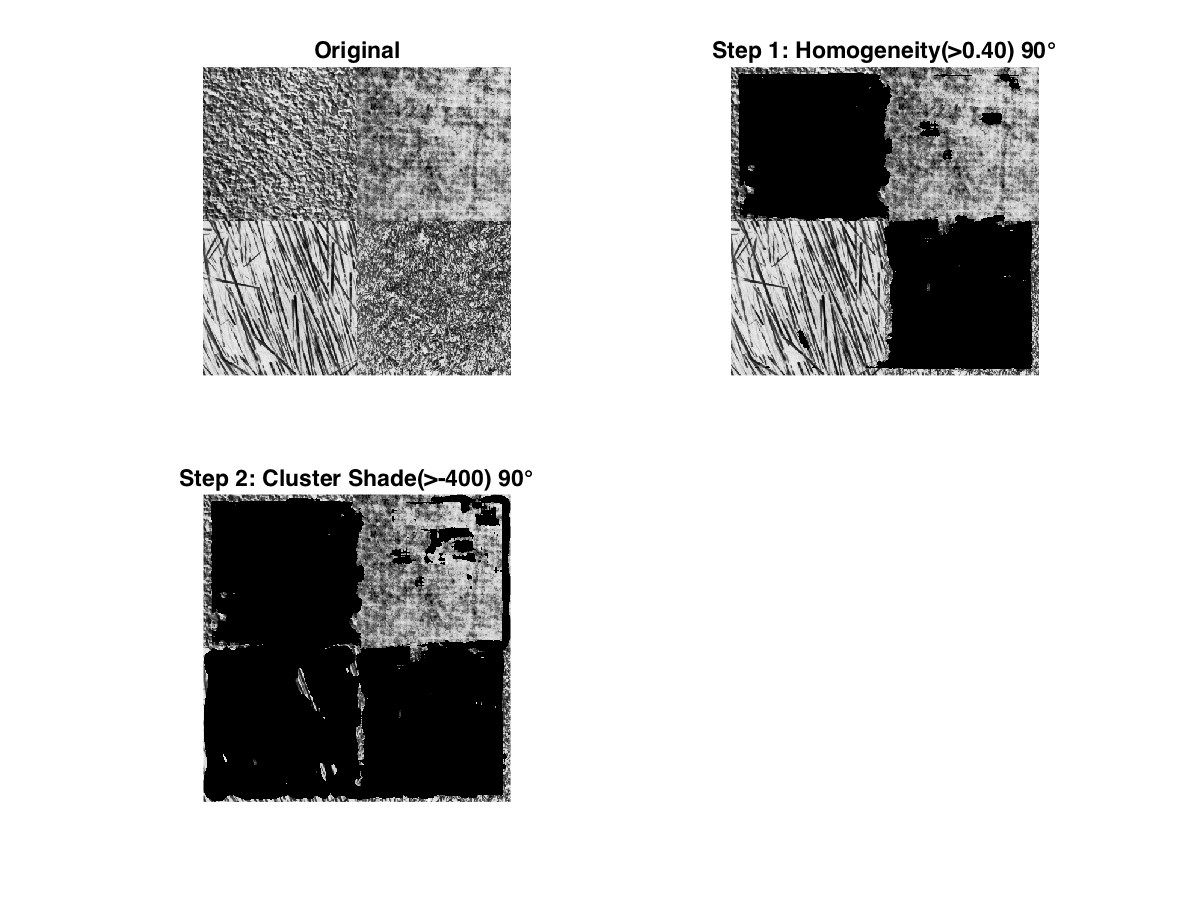
\includegraphics[width=0.8\textwidth]{partD-mosaic1-segmentation-top-right}
	\caption{Mosaic 1, top-right}
	\label{fig:Mosaic1SegmentedTopRight}
\end{figure}

\subsection*{Mosaic 1, Bottom-left} 
Segment \ref{fig:Mosaic1SegmentedBottomLeft}. Segmented using homogeneity at .40 and a \SI{90}{\degree} angle, followed by cluster shade at -400 using a \SI{90}{\degree} angle.

\begin{figure}[H]
	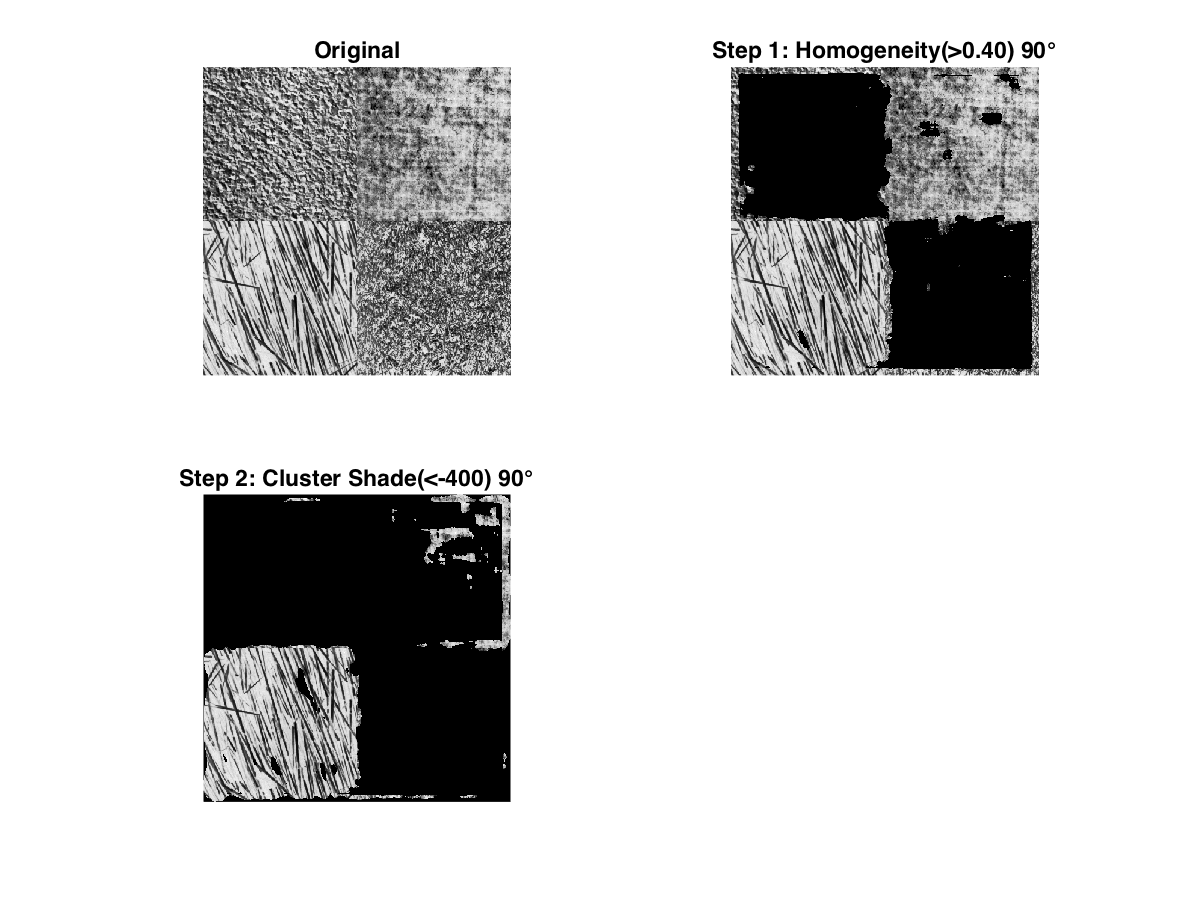
\includegraphics[width=0.8\textwidth]{partD-mosaic1-segmentation-bottom-left}
	\caption{Mosaic 1, bottom-left}
	\label{fig:Mosaic1SegmentedBottomLeft}
\end{figure}

\subsubsection*{Bottom-Right} 
Segment \ref{fig:Mosaic1SegmentedBottomRight}. Segmented using homogeneity at .40 and a \SI{90}{\degree} angle, followed by intertia at 13 using a \SI{45}{\degree} angle.

\begin{figure}[H]
	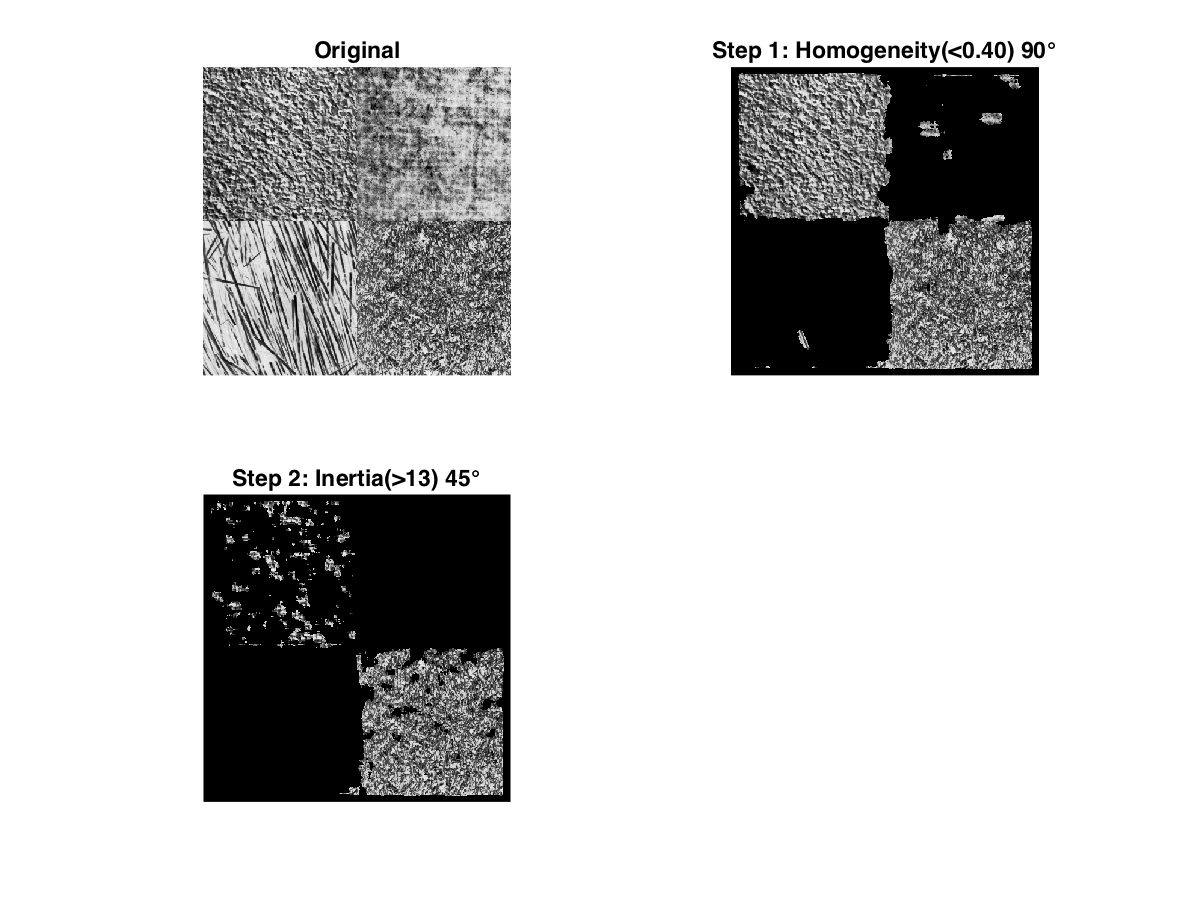
\includegraphics[width=0.8\textwidth]{partD-mosaic1-segmentation-bottom-right}
	\caption{Mosaic 1, bottom-right}
	\label{fig:Mosaic1SegmentedBottomRight}
\end{figure}



\subsection*{Mosaic 2, Top-left}
Segment \ref{fig:Mosaic2SegmentedTopLeft}. Segmented using homogeneity at .36 and a \SI{90}{\degree} angle, followed by intertia at 22 using a \SI{0}{\degree} angle.

\begin{figure}[H]
	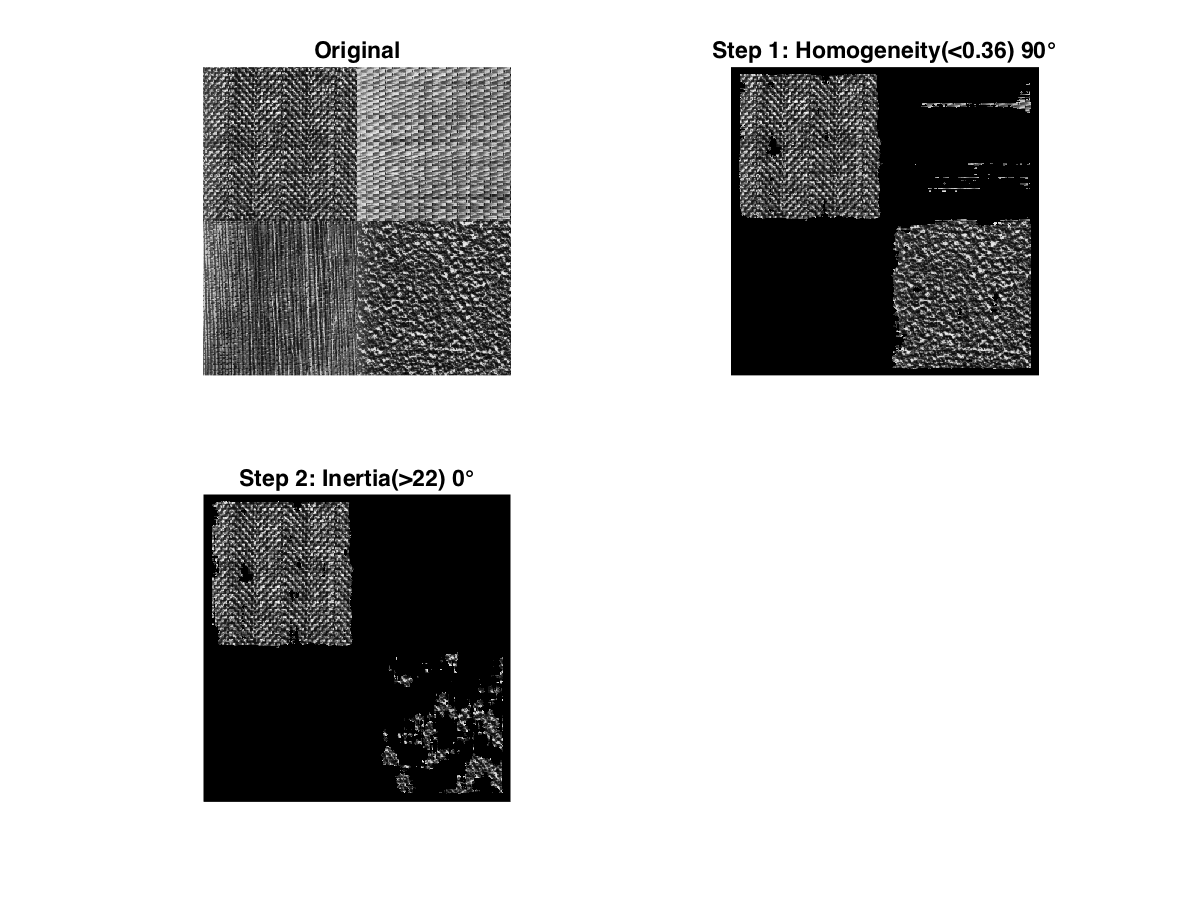
\includegraphics[width=0.8\textwidth]{partD-mosaic2-segmentation-top-left}
	\caption{Mosaic 2, top-left}
	\label{fig:Mosaic2SegmentedTopLeft}
\end{figure}

\subsection*{Mosaic 2, Top-right} 
Segment \ref{fig:Mosaic2SegmentedTopRight}. Segmented using homogeneity at .36 and a \SI{90}{\degree} angle, followed by intertia at 22 using a \SI{0}{\degree} angle.

\begin{figure}[H]
	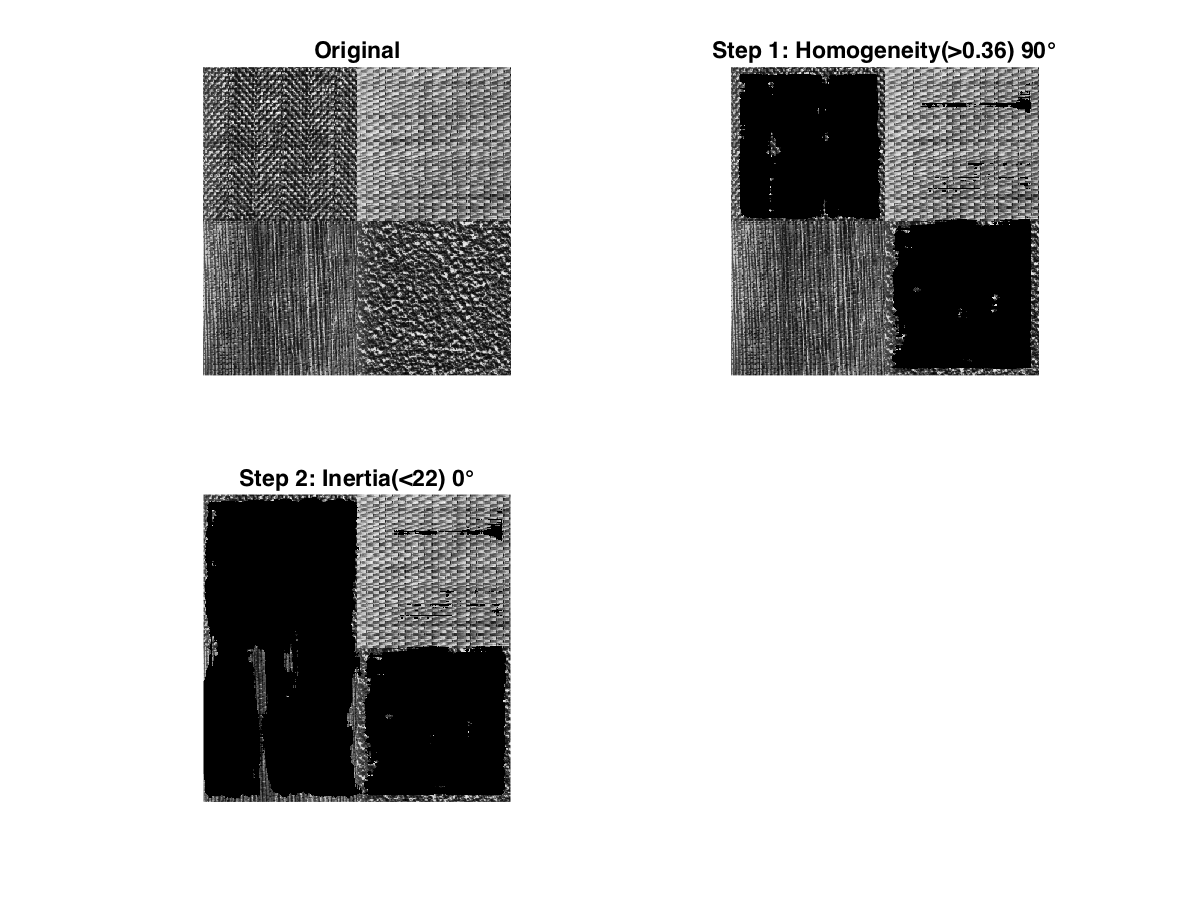
\includegraphics[width=0.8\textwidth]{partD-mosaic2-segmentation-top-right}
	\caption{Mosaic 2, top-right}
	\label{fig:Mosaic2SegmentedTopRight}
\end{figure}

\subsection*{Mosaic 2, Bottom-right} 
Segment \ref{fig:Mosaic2SegmentedBottomRight}. Segmented using homogeneity at .36 and a \SI{90}{\degree} angle, followed by intertia at 24 using a \SI{0}{\degree} angle.

\begin{figure}[H]
	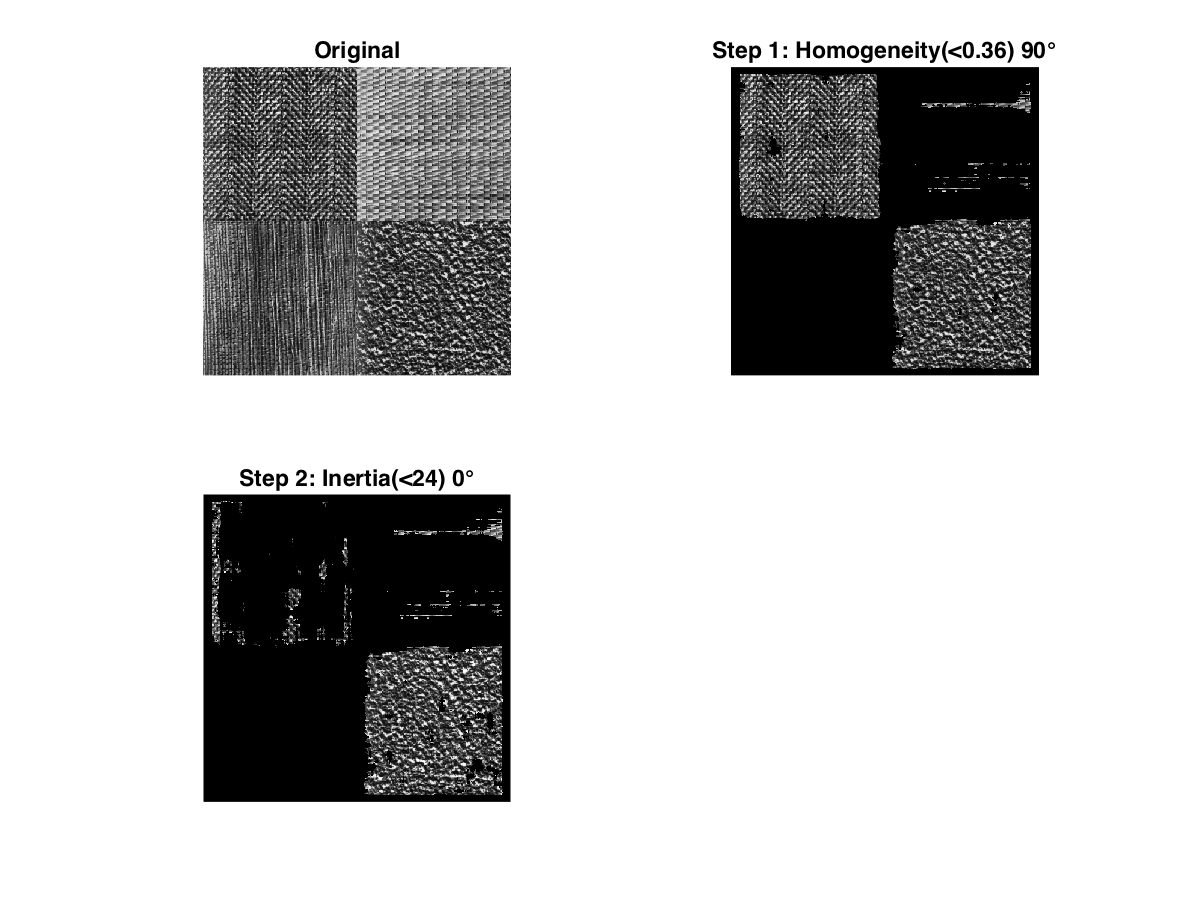
\includegraphics[width=0.8\textwidth]{partD-mosaic2-segmentation-bottom-right}
	\caption{Mosaic 2, bottom-right}
	\label{fig:Mosaic2SegmentedBottomRight}
\end{figure}

\subsubsection*{Bottom-Left}
Segment \ref{fig:Mosaic2SegmentedBottomLeft}. Segmented using homogeneity at .36 and a \SI{90}{\degree} angle, followed by intertia at 22 using a \SI{0}{\degree} angle.

\begin{figure}[H]
	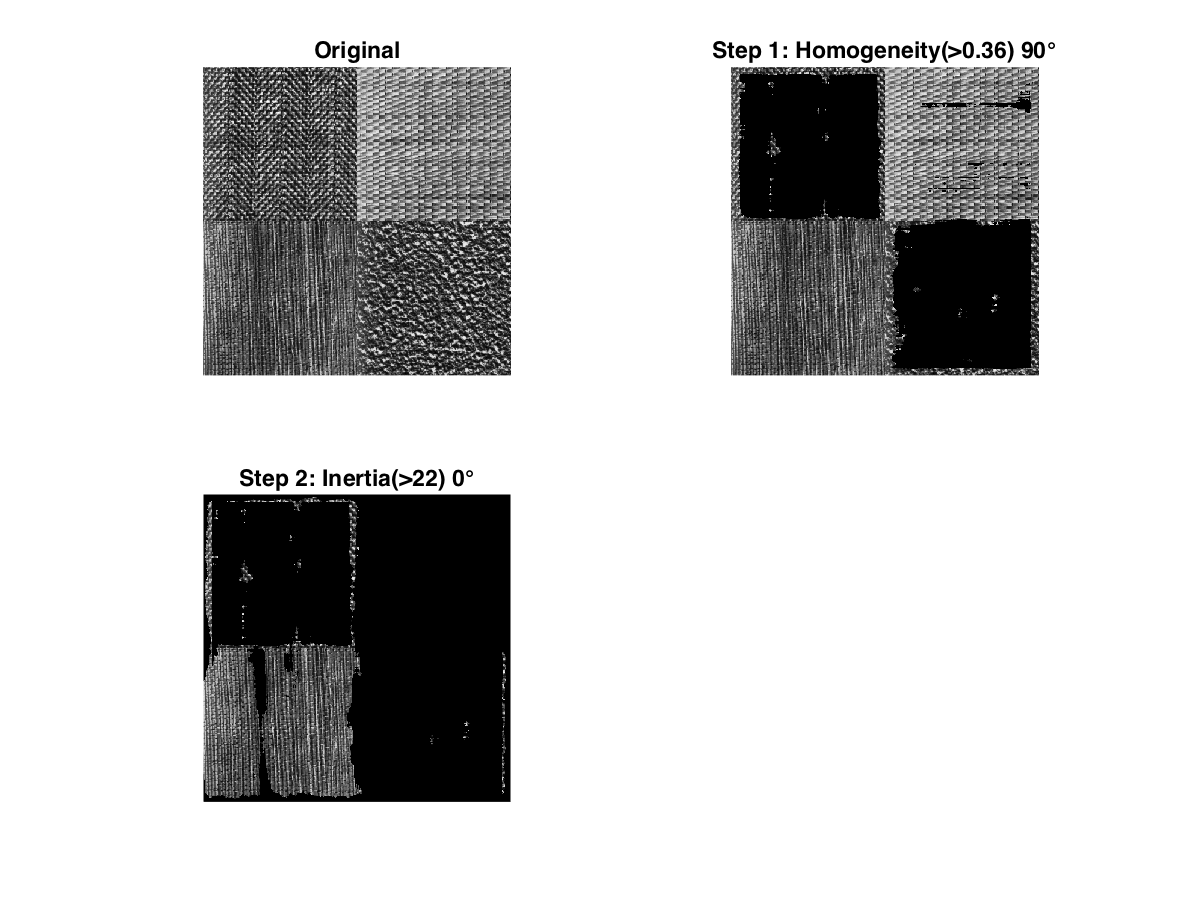
\includegraphics[width=0.8\textwidth]{partD-mosaic2-segmentation-bottom-left}
	\caption{Mosaic 2, bottom-left}
	\label{fig:Mosaic2SegmentedBottomLeft}
\end{figure}

\end{document}
